%!TEX root =  proposal.tex

\section{Computational biology applications}
\label{sec:compbio}



{\color{red}\large Cut this comp bio part of intro down to 1/2 or 1/3.  Should we remove it from intro and merge it into section 3?}

{\color{gray}
\paragraph{A computational biology stress test for our GPU data structures.}
Both the volume and variety of genomic sequencing data has been increasing at an ever faster rate, driven by new and improved massively parallel high-throughput sequencing (HTS) technologies.  These technologies are already producing
petabyte-scale datasets~\cite{kodama2012sequence}, and the NIH estimates that ``genomics research will generate between 2 and 40 exabytes of data within the next decade''~\cite{NHGRIDataScience}. Many applications in computational biology (\kmer
analysis~\cite{MarccaisKi11}, single-cell analysis~\cite{he2022alevin}, raw sequence search~\cite{solomon2016fast}, taxonomic classification~\cite{wood2014kraken}, and pangenomics~\cite{computational2018computational})
require processing raw sequencing data at petabyte scales~\cite{kodama2012sequence}. 
%
These applications are bottlenecked by the performance of an underlying core set of data structures, including filters~\cite{PandeyAlBe18, solomon2016fast}, hash tables~\cite{solomon2016fast,almodaresi2022incrementally}, locality sensitive hashing~\cite{Marais2019}, compressed string indexes~\cite{Almodaresi2018Pufferfish}, etc. % \mfc{fill in the rest from the remainder of intro, once we've read it.}. 
Specifically, the scale of the data is such that two main problems arise \textbf{(1)} some analyses are simply not currently feasible with existing data structures and algorithms --- for example, despite the long-standing desire to build a sequence-level index for the entire SRA, existing efforts have not reached this scale~\cite{Karasikov2020, HarrisM20, SolomonK17, almodaresi2022incrementally, AlmodaresiPFJP20,PandeyAlBe18} and \textbf{(2)} other common analyses are feasible, but computationally burdensome, requiring powerful local compute abilities, or leading to increased costs for analyses using cloud compute; this slows down the analysis and discovery cycle, and has led to a scenario in which, in many cases, compute has overtaken data generation as the predominant experiment-related cost~\cite{Muir_2016} (apart from humans). 

We identify two raw data analysis ``kernels''
that are used broadly throughout computational biology. These kernels are bottlenecks in many comp.~bio.~workflows, so making them faster and scaling them to larger data sets will have widespread impact. GPUs offer an avenue to scaling these data structures.  And while 
GPUs are fast, they are space constrained.  Therefore, we need new data structures and algorithms that are space efficient to speed up these applications.  
%
The kernels are:


\begin{itemize}%[leftmargin=*,nolistsep]
%\begin{itemize}[leftmargin=*,noitemsep,nolistsep]
\item \textbf{\Kmer analysis.}
\Kmer analysis involves representing raw sequencing data as length-$k$ subsequences called \defn{\boldkmers}, and performing analysis on the occurrence, frequency (and sometimes locations) of \kmers in the data sets; the objective is to answer questions about their genomic diversity, abundance variance, taxonomic information, etc. \Kmer analysis is the first step in numerous computational biology pipelines, e.g., error correction, de Bruijn graph construction, raw sequence search, digital normalization, comparative genomics, genomics assembly, transcript quantification, taxonomic classification of metagenomic reads, etc.~\cite{wood2014kraken,GeorganasEHG18,hofmeyr2020terabase,solomon2016fast,PatroSailfish:2014,PandeyAlBe18,PandeyBeJo17a,PandeyBeJo17b}.

Existing tools use both  approximate\footnote{In this proposal, we refer to data structures as \defn{approximate} if they  have only false positives and \defn{lossy} if they can have false negatives.} and exact data structures (e.g., filters vs.\ hash tables) to construct and store \kmer indexes~\cite{MarccaisKi11,PandeyBeJo17a}.  \Kmer analysis tools such as  Jellyfish~\cite{MarccaisKi11} use a compact filter to identify singleton \kmers and use a hash table to maintain the frequency count and associated metadata (e.g., prefix-suffix extension, read id, etc.) about the \kmers~\cite{hofmeyr2020terabase}. When the metadata is coherent, this can often be exploited to allow much more space-efficient indexing, at least in the static case~\cite{pibiri2022sparse,pibiri2023weighted,fan2023spt,fan2023fulgor}.
As we will see, \kmer analysis is a key part of several of the specific applications we will be addressing. 
%\mab{can somebody (else) name these? Alice, Bob, Eve?}

% \item \textbf{Compressed indexes.}
% FM-index, BWT, comressed suffix array.

\item \textbf{Sequence alignment.} Sequence alignment involves aligning sequences of DNA, RNA, or protein to identify similar regions that may be a consequence of underlying biological process and to establish evolutionary relationships.
Sequence alignment is used extensively in reference-based analyses, in which sequencing data is aligned against one or more reference genomes, as well as in genomic and metagenomic assembly to map contigs back to the reads during scaffolding. In computational biology applications, sequence alignment is often performed sequence to sequence; among multiple sequences (\emph{multiple sequence alignment}); and from a sequence to graph where the  graph is a \defn{sequence graph} representing genomes from multiple individuals.

 

Existing tools use compressed and succinct string indexes such as the BWT~\cite{burrows1994block} and FM-index~\cite{ferragina2000opportunistic}, the r-index~\cite{gagie2018optimal}, compressed suffix arrays~\cite{grossi2000compressed}, and several hashing-based schemes based on \kmers, minimizers, or other types of designed ``seeds''~\cite{li2018minimap2,pibiri2022sparse,sahlin2022strobealign}, as well as dynamic-programming algorithms for sequence alignment.
Compressed and succinct indexes support efficient ``seed'' lookup, which vastly reduces the set of candidate locations where a high-quality alignment might occur, and help to perform sequence alignment in a memory-efficient manner and enable these tool to scale to large volumes of data.
One of the most widely used tools across computational biology, BLAST~\cite{altschul1990basic}, performs fast and efficient sequence alignment using such string indexes.
%\mab{Shorten, or just improve writing on bullets}
%Given the large sizes of sequencing datasets, these tools also use hash-based \kmer indexes to seed the sequence alignment to achieve speedups.
\end{itemize}

\noindent
This toolbox is used, for example, to solve the following problems.

\begin{itemize}%[leftmargin=*,nolistsep]

\item \textbf{Taxonomic classification.} Taxonomic classification~\cite{wood2014kraken} helps to identify the microbial 
% \mfc{only microbial?} 
taxa present in large-scale metagenomic and microbiome datasets coming from complex biological and environmental samples by assigning a taxonomic label to each sequencing read. This plays an important role of many computational genomics pipelines for metagenomics projects, and is closely tied to the related problem of taxonomic abundance estimation (determining the taxonomic composition of a sequencing sample)~\cite{truong2015metaphlan2,skoufos2022agamemnon,wei2022kmcp}.

 

Methods for taxonomic classification of metagenomic data~\cite{wood2014kraken} often use hash tables to index the \kmer content of samples and quickly compare samples to prune the search space.
Furthermore, to save space, many solutions~\cite{wood2019improved} also employ approximate sketches (e.g., locality sensitive hashing (LSH)~\cite{roberts2004reducing, Marais2019}) to represent metagenomic data and perform similarity computations over sketches or reduced representations of the data~\cite{Shaw2023}.
Some approaches~\cite{kim2016centrifuge} employ compact string indexes such as the FM-index~\cite{ferragina2000opportunistic} to perform sequence comparison to determine exact matches among the pruned samples. There are many different tools for taxonomic classification.  Although they different in the details of their bottlenecks, they share some features: they are all bottlenecked around some aspect of $k$-mer analysis, especially around compression schemes for $k$-mer analysis.
%\mfc{which of these are bottlenecks?} \rob{to Martin's point/question --- there are \emph{many} different tools for taxonomic classification using different indexing strategies. Kraken (and Kraken2) are likely the most popular and use k-mer / minimizer hashing-based approaches. However, other pipelines like centrifuge and the recent Centrifuger use the FM-index or r-index. They provide different tradeoffs. Do we want to specifically lean into one here, or claim that we will tackle both?}.

 

\item \textbf{Raw sequence search.} Raw sequence search involves identifying all sequencing samples that contain a given query sequence in a database of raw sequencing data, such as SRA~\cite{kodama2012sequence}. A query is an arbitrary sequence, such as a gene transcript, or viral genome. Though common genomics processing pipelines extract and condense useful information (e.g., genomic variants, transcript abundance, etc.) from raw sequencing data, current solutions often eliminate unexpected signal or diversity (e.g., specific viral or microbial reads that might be present across many samples~\cite{Edgar2022}). 
%\mfc{to be clear: this is a false-negative issue, not a performance issue}

 

Methods for raw sequence search use \kmer-based indexing tools to build an inverted index from the \kmers to the underlying samples where the \kmer is present. Tools such as SSBT~\cite{solomon2016fast} build a tree of approximate \kmer indexes to quickly prune the search space of samples. Other tools include:  Mantis~\cite{PandeyAlBe18}, which builds an exact inverted index that uses compact hash tables; or Metagraph~\cite{Karasikov2020}, which uses a \kmer-index based on a succinct representation of the de Bruijn Graph~\cite{bowe2012succinct}.

 

In raw sequencing data, singleton \kmers are most likely caused by sequencing errors, yet they make up a large fraction of the data~\cite{solomon2016fast,MarccaisKi11}. These tools often use filters to weed out singleton \kmers.

%\mfc{I still don't know what the bottleneck is.}

%\mab{So far, the proposal does a great job of convincing people that we are experts. And that requires most of the real estate. What still needs to happen is (1) we need to convince the reader that actual pain is experienced, and (2) we need to convince the reader that we have a solution to this pain. Only a small number of additional sentences, but necessary ones. We haven't even mentioned GPUs as a possible solution.}

 

\item \textbf{Pangenomics.}
Pangenomics~\cite{garrison2018variation} involves representing the biological variation represented within and across populations of individual organisms belonging to a species or group.  The most popular approaches to pangenomics store the genome of a species as a sequence graph consisting of genomes of multiple individuals (or multiple major haplotype groups) instead of a single linear reference. A primary goal of pangenomic variation analysis is to avoid biases that arise when treating a single genome as the reference when identifying or comparing variants across samples in a population.

 

Existing tools for constructing a pangenomic graph use a combination of succinct data structures (e.g., compressed bit vectors~\cite{garrison2018variation}), space-efficient, dynamic hash tables, and string data structures~\cite{pandey2021variantstore}.

% \prashant{Talk about Metahipmer here.}

\end{itemize}

%\mfc{this sounds like software engineering.  why is there a technical problem?   are we just having them pay for us to build stuff that no one has gotten around to building?  Still no discussion of what the challenges are.}

Our goal 
is to build tools for performing complex biological analyses at the scale of terabytes and petabytes, for datasets that are available today, and beyond, for the datasets of the future. For example, raw sequencing data from SRA~\cite{kodama2012sequence} is already at petabyte scale, metagenomic data from WA and Rhizo~\cite{hofmeyr2020terabase} are hundreds of terabytes, and pangenomic data from the 100,000 Genome Project~\cite{1002021100} are sequencing individuals at population scale. To quickly process and perform biological analysis on these data we will exploit the massive computing in modern GPUs (e.g., NVIDIA's Tesla V100 and A100) and also the distributed computing infrastructure of supercomputers (Perlmutter~\cite{perlmutter} and Summit~\cite{summit}).

\textbf{The computational biology applications described above (and numerous others)  use a set of common data structures to perform data-analysis tasks.}
Compact and exact data structures include: hash tables and succinct bit vectors, compressed string indexes, and trees.
Sketches and approximate data structures include: filters, cardinality estimators,  min-hash based sketches, and other locality-sensitive hash data structures.

% \setlength\intextsep{0pt}
\begin{wrapfigure}{R}{0.6\textwidth}
% \begin{figure}
\centering
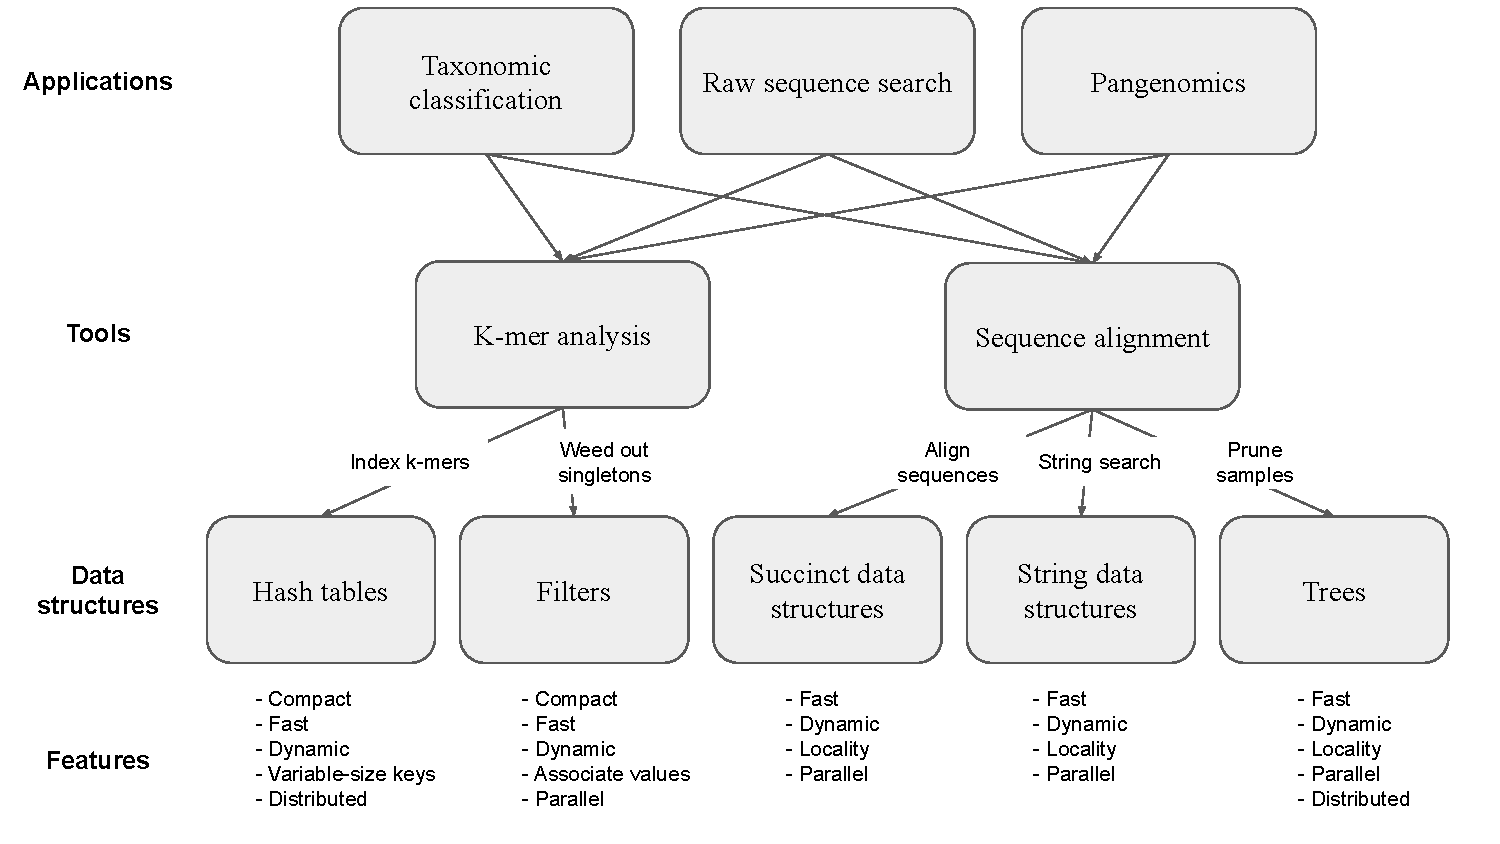
\includegraphics[width=1.0\textwidth]{images/PPOSS_App_DS}
\caption{Relation between computational biology applications, data processing tools and data structures. We further mention the desired features in data structures to achieve performance and scalability.}
\label{fig1}
% \end{figure}
\end{wrapfigure}

The performance and scalability of the computational biology applications
depends on the space-efficiency, speed, dynamism, and scalability of the
underlying data structures they use. These data structures are also the building blocks in many other domains, such as databases, machine learning, software systems, and security applications.




% \mfc{this next paragraph feels redundant.  PRashant, do we just kill it?}

% \paragraph{Existing software tools for computational biology applications.}
% \sout
% {There are numerous tools for \kmer counting~\cite{MarccaisKi11,PandeyBJP17a}, sequence alignment~\cite{altschul1990basic,kielbasa2011adaptive,li2018minimap2,schwartz2003human}, raw sequence search~\cite{solomon2016fast,PandeyABFJP18Cell}, taxonomic classification~\cite{wood2014kraken,wood2019improved}, and pangenomics~\cite{garrison2018variation,pandey2021variantstore}. These tools rely on space-efficient and high-performance CPU data structures such as filters, sketches, hash tables, and string indexes. Most of these tools are designed for shared-memory parallelism and they often do not scale out of shared memory to disks.
% These existing tools are limited by single-node compute and shared-memory parallelism. They are not designed to scale to thousands of cores on modern accelerators nor scale out to hundreds to nodes in a high-performance computing (HPC) environment.
% }
%


\label{sec:we-need-performance-and-scalability}
\paragraph{CPU speed and RAM capacity cannot keep up with data growth.}
Unfortunately, CPU speed and RAM sizes aren't keeping up with the data growth in computational biology and other applications.
Although CPU performance is increasing at 2--25\%/year and single-node RAM sizes are increasing at 2--11\%/year, genomics data is is likely to double in size every 1.5 years~\cite{kodama2012sequence}.
% See~\Cref{fig:sra_data}.
Thus, today's software tools will not scale with tomorrow's data. For example, performing \kmer analysis or sequence alignment on petabyte-scale raw sequencing data is not possible on single-node shared-memory systems.

In the post-Moore’s-Law period, performance gains will come from software, algorithms, and hardware rather than semiconductors~\cite{leiserson2020there}. We can achieve massive scalability by first, designing data structures and algorithms to scale up using modern accelerators such as GPUs and second, scaling out by using distributed memory in an high-performance computing (HPC) environment.



\paragraph{GPUs and other accelerators in computational biology.}
As with other high-performance computing (HPC) domains,
GPUs are increasingly used in large-scale computational biology applications because they offer a substantial jump in terms of low-cost parallelism, as long as data structure and algorithms can be designed and implemented to match the memory and parallelism requirements of GPUs.
%
For example, GPUs are already used in some recent computational biology applications to speed up \kmer counting~\cite{nisa2021distributed} and local assembly~\cite{awan2021accelerating}.

However, the penetration of GPUs into biology pipelines is limited by how the limitations of GPUs have translated so far into data structures.  These GPU limitations include:
\begin{enumerate}%[leftmargin=*,noitemsep,nolistsep]
  \item GPU device RAM is much smaller than CPU RAM\@; this is especially
    challenging given the data sizes in computational biology.
  \item GPUs have high contention due to thousands of threads and are
    inefficient when computations are irregular.
  \item GPUs don't have a fully functional, high-performance suite of memory management tools; it is hard to perform dynamic memory management without involving the host CPU\@. 
  % \john{I'm not sure what the main point is here; dynamic memory management is not terrible on GPUs~\cite{Winter:2020:OVQ}, though it does have limitations. I softened this. But I don't get this point.}
\end{enumerate}

These limitations affect the capabilities of GPU data structures: most existing GPU data structures do not support dynamic resizes and are statically allocated; pointer-based data structures such as trees and tries do not achieve high performance on GPUs; data structures on hard-to-align data, such as strings or vectors, which have variable lengths are not available; and GPU data structures do not scale out of the GPU's device RAM to host.

These limitations are critical for building scalable computational biology applications. For example, in \kmer analysis during raw sequence search and taxonomic classification, the size of the \kmer multiset is not known in advance. thus, applications initialize the data structures  to a default size and then dynamically resize (mostly expand) based on the actual number of \kmers. The ability to resize is critical to space-efficient \kmer analysis. Static data structures such as hash tables and filters~\cite{GeilFO18} currently available on GPUs are sized using an overapproximation of the number of \kmers, which leads to space inefficiency.
Similarly, the local assembly module involves constructing thousands of hash tables in parallel and then using them to perform contig (contiguous strand of DNA) extension walks. The CPU implementation of local assembly relies on dynamic
structures such as hash tables, vectors and strings, which are a challenge to implement on GPUs. In addition, local assembly induces a random memory-access pattern with a non-deterministic amount of work, which further complicates implementing this module on GPUs.

% \begin{wrapfigure}{r}{0.45\textwidth}
% \centering
% 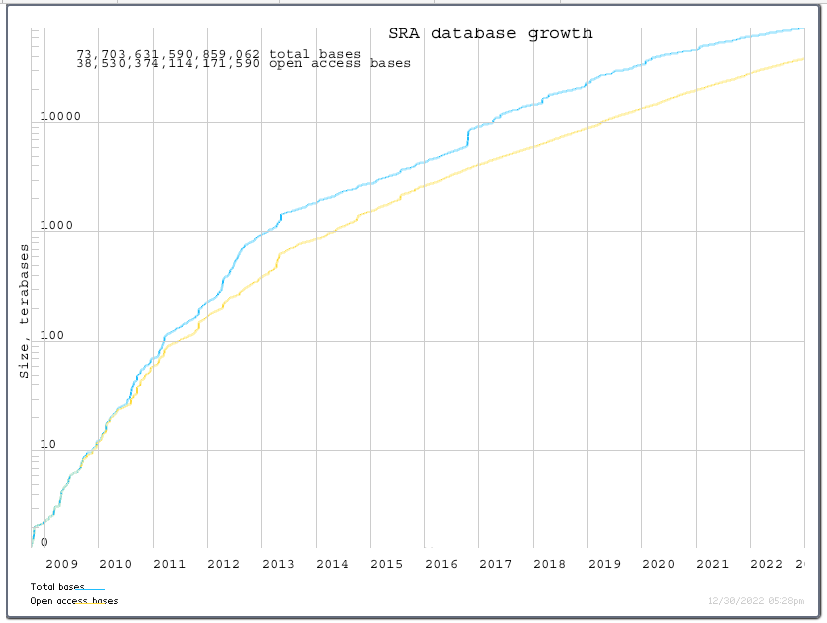
\includegraphics[width=0.95\textwidth]{images/SRA_data_growth.png}
% \caption{Sequence read archive (SRA) data growth. SRA data contains a trove of biological diversity information. Existing computational biology tools do not scale to support searching through all of SRA\@. This renders what is otherwise an immensely valuable public resource largely inert.}
% \label{fig:sra_data}
% \end{wrapfigure}


% GPUs have not seen widespread adoption in computational biology applications. For example, they are used in taxonomic classification of metagenomic data, indexing and searching through terabytes of raw sequencing data, constructing and querying pangenomic graphs.

%Anything that involves sophisticated data structures and when memory is constrained GPUs are not currently useful.

% GPUs are not currently used for many computational biology applications because efficient GPU data structures do not exist.

\para{Requirements for building scalable computational biology applications}
Data structures are the core of computational biology applications and are critical for their performance and scalability.
To build scalable computational biology applications that can keep up with the rapid growth data we need compact, high-performance, dynamic, and distributed data structures. Specifically, we need: (1) approximate data structures such as filters, sketches, and locality-sensitive hashing data structures; and (2) exact data structures such as hash tables, string data structures, succinct data structures, and trees.

These data structures and algorithms will need to exploit accelerators such as GPUs to scale up computations and at the same time support  features such as space-efficiency, dynamism, high concurrency, scaling out of GPU device RAM to host RAM, and distributed memory design to scale out to multiple nodes.
%
Furthermore, to achieve fine-grained resizing and to keep the peak memory usage low, we first need to develop new algorithmic approaches for traditional CPU data structures and then extend them to GPUs.
}


\subsection{Taxonomic classification and abundance estimation of metagenomic data}

\textbf{Problem definition.}
% The microbes that live in an environment can be identified by their combined genomic material, also called the metagenome. 
Metagenomic datasets contain sequencing reads from multiple species (and strains) that are present in the environment from which the sample was drawn. Metagenomes provides an opportunity to closely examine complex  interactions, such as phage-host and metabolic dynamics~\cite{national2007new}.
%
Taxonomic classification~\cite{wood2014kraken} helps to identify the microbial taxa present in large-scale  metagenomic datasets. Assigning taxonomic labels to sequencing reads, and the related challenge of quantifying the associated abundances of these taxa, are important steps in many computational genomics pipelines for metagenomics projects.

\noindent
\textbf{Importance.}
Metagenomic sequencing produces genomic data from a collection of species instead of an individual isolate. One of the primary challenges in the field is the development of computational methods for identifying the species contained in these samples, and accurately estimating their associated abundances.
%
Taxonomic classification of reads is a critical first computational step in any metagenomic analysis pipeline. For example, read classification is critical for \emph{de novo} metagenomics assembly, which attempts to reconstruct the DNA sequence of each organism present in the metagenomic sample without using a reference database before performing the actual assembly step~\cite{venter2004environmental,brady2009phymm,brady2011phymmbl,rosen2008metagenome,segata2012metagenomic}.  Likewise, the related task of taxonomic abundance estimation is a critical step in understanding how micriobial abundances change over time, between conditions of interest, or in response to a stimulus or treatment~\cite{Kaehler2019,wei2022kmcp,skoufos2022agamemnon,BlancoMguez2023}. While these tasks are highly-related, they represent distinct challenges, as taxonomic read assignment asks for a deterministic assignment of each read to some taxon (perhaps at some aggregated taxonomic level), while taxonomic abundance estimation asks for an estimate of the abundance of the different taxa in a sample, allowing the probabilistic or proportional allocation of individual sequencing reads.

\noindent
\textbf{Challenges.}
The task of read classification is far from straightforward.
A metagenomic sample can contain thousands of genomes with varying level of similarities and often occurring at vastly different abundances. Furthermore, due to high-throughput sequencing, metagenomic samples contain millions of sequencing reads making traditional, string-matching-based tools like BLAST~\cite{altschul1990basic} infeasible to perform classification. Metagenomic datasets today easily range from hundreds of GBs to TBs~\cite{hofmeyr2020terabase}, e.g., the WA dataset contains a collection of marine microbial communities from the Western Arctic Ocean and consists of 822~GB of 2.5 billion reads in 12 samples~\cite{hofmeyr2020terabase}.
%
Although BLAST is one of the most sensitive metagenomics alignment methods, it is computationally intensive, making it infeasible to run on the millions of reads present in metagenomic sequencing studies.

\noindent
\textbf{State of the art.}
Many recently developed taxonomic classification tools~\cite{ames2013scalable, kim2016centrifuge, menzel2016fast, wood2014kraken, wood2019improved, dilthey2019strain,liu2018novel} use a supervised approach to assign taxonomic labels to reads.
These tools build a database of previously sequenced microbial genetic sequences and their taxonomic labels from the NCBI database.
The database is usually a compact hash table that maps smaller subsequences (\kmers) to the list of taxa corresponding to the genomes in which the subsequences occur.
Then, the input reads are decomposed into \kmers and queried in the index to determine the most appropriate taxon using the lowest-common ancestor (LCA) of the genomes in the taxonomic tree.

\noindent
\textbf{Gaps and requirements.}
The size of sequenced microbial genetic sequences presents a computational and memory challenge.
% Building the database of known genomes is often quite memory intensive.
The most popular reference database are RefSeq complete genomes (RefSeq CG) for microbial species and the BLAST nt and nr databases for high-quality nucleotide and protein sequences, respectively, with $\approx50$ and $\approx200$ million sequences.
Kraken's~\cite{wood2014kraken} memory requirements can easily exceed 100~GB~\cite{simon2019benchmarking}, especially when the reference data includes large eukaryotic genomes~\cite{meiser2017sequencing, knutson2017porcine}.
%
The universe of microbial sequences is large and diverse. The vast search space often results in false positives as sequences can be matched against multiple taxa. Also, a large number of undiscovered microbial species can result in false negatives as these species are not present in the database.

Existing taxonomic classification tools are memory intensive to build the database of known genomes and often require more memory than available on single-node machines. Furthermore, the classification operation is computationally intensive, making it infeasible to scale to terabyte-scale metagenomic datasets.
Second, this challenge is compounded by the exponential growth in recent years of the number of sequenced microbial genomes, meaning that the number of comparisons that need to be performed for new sequencing reads is huge and ever-increasing.
%
Finally, existing reference database indexes give up updatability to save space. However, the ability to add new assembled genomes to an existing database is a critical feature to avoid rebuilding the databases.


\begin{rproblem}[\textbf{Metagenomic classification at terabyte scale}]
Build a software tool to perform reference-based taxonomic classification of metagenomic reads for terabyte-scale metagenomic datasets. The software tool will support adding newly sequenced microbial genetic sequences to the database and updating the labels of existing ones without rebuilding the whole database.
\label{rprob:taxo-meta}
\end{rproblem}

% \mfc{there is no discussion of what we are actually going to do.  what hardware?  what tests?  how will we know that we succeeded?  How much of an improvement do we need in order to succeed?  What it will it mean to our target application community if we succeed?}


\subsection{Large-scale raw sequence search}

\textbf{Problem statement.} Raw sequence search involves identifying all sequencing samples in a database of raw sequencing data such as SRA~\cite{kodama2012sequence,KatzSLKBO22} that contain a given query sequence. A query is an arbitrary sequence, such as a transcript. Raw sequencing datasets contain a ton of biological diversity information that can be used to answer biological questions that single-sequencing samples do not have the power to address.

\noindent
\textbf{Importance.}
The Sequence Read Archive (SRA)~\cite{kodama2012sequence}, the world’s largest database of sequences, hosts approximately 10 petabytes %(1016 bp) 
of sequence data and is growing by 
%at the alarming rate of 
10 TB per day.
%
The vast majority of publicly available sequencing data (e.g., the data deposited in the Sequence Read Archive, or European Nucleotide Archive (ENA)~\cite{CumminsAABDEGHH22}) exist in the form of raw, unassembled sequencing reads. The raw sequencing data contains a lot of biological diversity information which is lost during the assembly process. Furthermore, only a small fraction of all the raw sequencing data is assembled, making the raw sequencing data even more important to answer complex biological-diversity related questions.
%
Enabling scientists to analyze existing sequence data will provide insight into ecology, medicine, and industrial applications~\cite{LeviRAE18}.
%
The genomics community established this database to enable sharing of the data, but the computational barrier to searching this data leaves it separated from the people most qualified to analyze it.

\noindent
\textbf{Challenges.}
Many tools, such as BLAST~\cite{altschul1990basic} and its variants, have been designed to perform sequence-level searches over publicly available databases of assembled genomes and known proteins. %Much subsequent work has focused on how to extend tools such as BLAST to be faster, more sensitive, or both~\cite{XXX}. \mfc{This previous sentence is a jolt. what does that have to do with raw sequence data?}
However, such tools focus on the case where queries are issued over a database of reference sequences which is much smaller in size compared to the SRA\@.
Using BLAST (or other BLAST-based tools) to perform searches over SRA is computationally infeasible.
%
There are a number of reasons that typical reference-database-based search techniques cannot easily be applied in the context of searching raw, unassembled sequences. One major reason is that most current techniques do not scale well as the amount of data grows to the size of the SRA (which today is $\approx4$ petabytes of sequence information). A second reason is that searching unassembled sequences means that relatively long queries (e.g., genes) are unlikely to be present in their entirety as an approximate substring of the input.
As such, these data have mostly been rendered impervious to sequence-level search, which substantially reduces the utility of such publicly available data.


\noindent
\textbf{State of the art.}
New computational schemes have been proposed that promise to search raw SRA while overcoming these challenges. Solomon and Kingsford~\cite{solomon2016fast} introduced the sequence Bloom tree (SBT) data structure and an associated algorithm that enables an efficient search over thousands of sequencing experiments. Specifically, they re-phrase the query in terms of \kmer set membership in a way that is robust to the fact that the target sequences have not been assembled. The resulting problem is coined as the \emph{experiment discovery problem}, where the goal is to return all experiments that contain at least some user-defined $q$ fraction of the \kmers present in the query string.
%
Subsequently, Mantis~\cite{PandeyAlBe18} was developed by PI Pandey, Patro and Bender that showed how to solve the experiment discovery problem using an inverted-index approach by mapping \kmers to the list of experiments in which they appear. Mantis uses the counting quotient filter~\cite{PandeyBJP17} developed by PI Pandey as a space-efficient and exact map to map \kmers. Mantis's index is smaller in size, faster to index and query, and has no false positives compared to the SBT (and other SBT-based tools~\cite{SolomonK17,HarrisM20,BingmannBGI19}).
%
PIs Pandey and Patro further continued this effort to compress the Mantis index in order to reduce memory requirements and scale Mantis~\cite{AlmodaresiPFJP19,AlmodaresiPFJP20} out of RAM to storage devices.


\noindent
\textbf{Gaps and requirement.}
Existing raw sequence search indexes suffer from the scalability challenge. Indexing \kmers from the SRA samples is memory-intensive and indexes often take hundreds of GBs. For example, the SBT index size for 2652 experiments consisting of short-read RNA sequencing runs of human blood, brain, and breast tissues is 97~GB\@. Scaling SBT-based indexes to 100K experiments in SRA is not currently feasible on single-node machines and scaling to an approximation of the entire SRA is likely not possible on a single machine, even with improved representations.
Furthermore, SBT-based indexes are approximate; the search results include false positives, which can quickly become problematic even if only 1\% of results are false positives, due to the sheer size of the search space.

Mantis's index is exact and has no false positives. Recently, LSM-Mantis~\cite{almodaresi2022incrementally} showed how to efficiently scale the index to SSD storage devices using Bentley/Saxe's transformation~\cite{BentleyS80}. However, even LSM-Mantis could only index 40K experiments from the SRA\@. These indexes are reaching the limits of single-node RAM and storage hardware.

Finally, in addition to representing the exact (or approximate) \kmer sets, a key challenge in constructing a large-scale sequence search index is the ability to build a compact yet updatable color-class representation. The \emph{color} of a \kmer is the set of indexed samples in which it is present; (conceptually, this can be thought of as a simple list of samples for each \kmer, or a binary vector with dimension equal to the number of indexed samples;) 
since many \kmers share exactly the same patterns of occurrence across samples we can instead discuss color-classes --- the distinct subsets of occurrence where two \kmers are deemed equivalent under the color relation if they appear in exactly the same set of samples.  In existing work, there is a substantial tension between the overall size of the representation of the color-class information, and the ability to add to or update this representation, with highly-compressed representations existing~\cite{Karasikov2020,Pibiri2023MacDBG,AlmodaresiPFJP19}, but being restricted mostly to static or semi-static indexes.  In this proposal, we will seek to leverage our work on building dynamic succinct data structure primitives to develop novel, compact, and \emph{updatable} color-class representations, drawing on ideas from our prior work in compact static representations~\cite{AlmodaresiPFJP19,Pibiri2023MacDBG}.

% \prashant{Add a discussion about representing color-classes.}

\begin{rproblem}[\textbf{Build a raw sequence search index over all of SRA}]
Build a \kmer index over all the raw experiments present in SRA and enable sequence-level searches in real-time. Furthermore, host the index publicly to make it available for researchers around the world.
% Researchers can quickly ask biological questions and get answers.
% For example: what if researchers wants to determine: if a new putative disease-related transcript appeared in other samples, if a new fusion event is common among samples with a given subtype, which samples contain a new unexpected bacterial contaminant.
\label{rprob:seq-search}
\end{rproblem}

\subsection{Pangenomics}

\textbf{Problem definition.}
Pangenomics~\cite{sherman2020pan} involves cataloging the DNA of multiple individuals in a species in the form of a sequence graph to preserve the variation across the individuals in a species. This pangenome is used as the reference genome for the species and forms the basis of thousands of studies seeking the genetic origins of diseases. In pangenomics, we need to efficiently index the variations (SNPs, indels, copy number, structural, etc.) and support variant queries. Furthermore, we need to perform sequence-to-graph alignment to determine new variants.


\noindent
\textbf{Importance.}
Much of the field of genomics revolves around the existence of reference genomes, which are roadmaps for a ‘typical’ individual of each species.  However, as the number and scope of sequencing experiments have grown dramatically, scientists have begun to realize the many limitations that a single reference genome imposes upon the community. To better capture the variation missed by using one reference, we can create and utilize a ‘pangenome’, a collection of all the DNA sequences that occur in a species.
A primary goal of pangenomic variation analysis is to avoid biases that arise when treating a single genome as the reference when identifying or comparing variants across samples in a population. 
The first pangenomes were developed for small, easy-to-sequence bacteria, but, even in that context, pan-genomes provided novel scientific insights. The consideration of genetic diversity within bacterial species has contributed to our understanding of underlying differences in pathogenicity, virulence and drug resistance and can even help predict how pathogenic a new strain will be~\cite{sherman2020pan}.

\noindent
\textbf{Challenges.}
Cataloging the DNA from all individuals in a species is a daunting task.
Building a pangenome graph involves storing the genomic sequences of thousands individuals in the form of a sequence graph. Each path in the sequence graph follows the genome of an individual and has a unique coordinate system. A coordinate systems helps to identify the location of a variant in the genome of an individual. Due to the presence of insertions and deletions in genomes across individuals, each individual can have a unique coordinate system~\cite{pandey2021variantstore}.
During variant queries, we need to identify a variant with respect to an individual's coordinate system due to the absence of a reference genome.
A Pangenome consists of thousands of individuals and hence thousands of coordinate system in a single index. Indexing and querying the pangenome graph across thousands of coordinate system is computationally and memory intensive and requires scale up and scale out solutions~\cite{garrison2018variation,pandey2021variantstore}.

\noindent
\textbf{State of the art.}
Pangenomic studies are performed by storing the genomes of multiple individuals in a genome graph (also known as the sequence graph or variation graph). A genome graph is a directed, acyclic graph (DAG) $G = (N, E, P)$ that embeds a set of DNA sequences. It comprises a set of nodes $N$, a set of direct edges $E$, and a set of paths $P$. For DNA sequences, we use the alphabet \{A, C, G, T, N\}\@. Each $n_i \in N$ represents a sequence $seq(n_i)$. Edges in the graph connect nodes that are followed on a path. Nodes on a path are assigned positions based on the coordinate systems of sequences they represent.

% Efficiently indexing and storing a genome graph is a computationally and memory/space intensive process due to the presence of thousands of coordinate systems corresponding to the individuals.
Existing applications that index genome graphs~\cite{pandey2021variantstore,garrison2018variation} are designed to use compressed string indexes and off-the-shelf graph indexes. VG toolkit~\cite{garrison2018variation} is one of the most widely used tools to represent genomic variation data, and it also supports multiple coordinate systems. VG toolkit stores each sample path as a list of nodes in the graph and maintains a separate index corresponding to the coordinates of the reference and samples.
%
PI Pandey developed VariantStore~\cite{pandey2021variantstore}. It encodes genomic variation in a directed, acyclic variation graph and build a position index (a mapping of node positions to node identifiers) on the graph to quickly access a node in the graph corresponding to a queried position. It builds an inverted index from variants to the nodes in the graph to achieve space efficiency due to repeated variants and fast variant queries.

\noindent
\textbf{Gaps and requirement.}
Current pangenomic indexes do not scale to population-scale variation datasets such as 100,000 Genomes project~\cite{1002021100}. For example, VG toolkit stores each sample path as a list of nodes in the graph and maintains a separate index corresponding to the coordinates of the reference and samples. Storing a separate list of nodes for each sequence impedes the scalability of the representation for storing variation from thousands of samples. Moreover, variants are often shared among samples, so storing a list of nodes for each sample path introduces redundancy in the representation.
%
Existing pangenome indexes do not support adding new genomes to an existing index. In order to add a new genomic sample to the pangenomic index required rebuilding the complete index. For example, both VG toolkit and VariantStore are static indexes and do not support an efficient approach for adding new genomes to an existing index.

Finally, pangenomic indexes need to support fast variant queries and sequence-to-graph alignment. Achieving both these operations in a single index is a challenging task. Existing tools are optimized for one of these operations but not both. VG toolkit is designed for fast sequence-to-graph alignment and VariantStore for variant queries.


\begin{rproblem}[\textbf{Building a pangenomic index at population-scale }]
 Build a pangenomic index that can perform fast variation queries and sequence-to-graph alignment at population-scale datasets available today. We further want to support adding new genomic samples to an existing index without rebuilding the index.
\label{rprob:pangenomics}
\end{rproblem}


\if 0
\subsection{Metagenome assembly}

% \begin{figure}
% \begin{wrapfigure}{R}{0.7\textwidth}
%     \centering
%     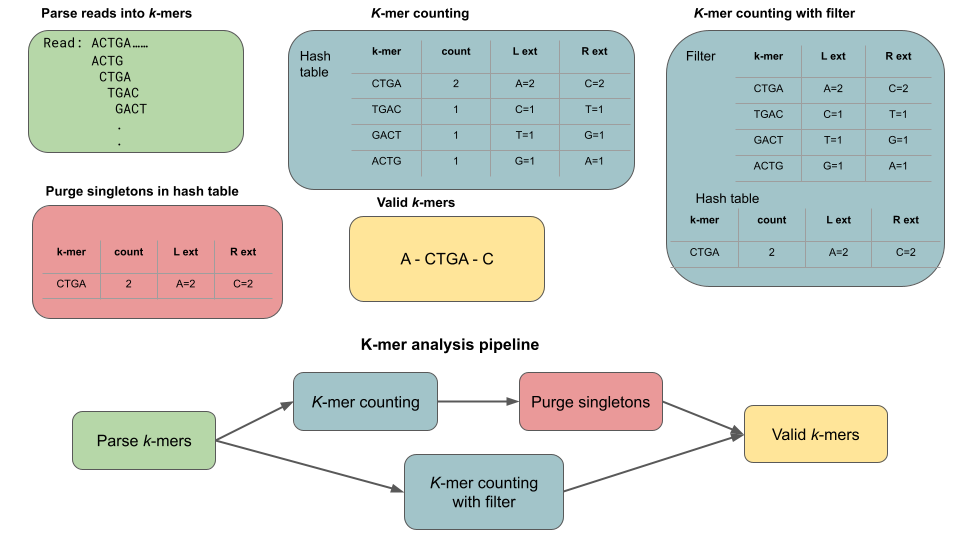
\includegraphics[width=0.9\linewidth]{images/mhm-pipeline.png}
%     \caption{The \textit{k}-mer analysis pipeline in MetaHipMer. A filter can help weed out singleton \kmers from being inserted into the hash table.}
%     \vspace{-0.5em}
%     \label{fig:mhm-kmer}
% \end{wrapfigure}
% \end{figure}

\textbf{Problem definition.}
Metagenome assembly involves reconstructing long contiguous sequences (\emph{contigs}) of genetic material from short input \emph{reads}~\cite{yang2021review}. These reads are strings of bases (the DNA alphabet A, C, G, T) of length 150 to 250 that are produced by gene sequencing machines.
For metagenomes, these reads are extracted from environmental samples (e.g., gut bacteria, or a soil sample) that contain the genes of potentially thousands of microbes, existing at varying abundances.
The reads are error-prone (typically about 0.24\% error per base) and sequencing is done multiple times to ensure every region of genetic material is covered with some error free sequences.

\noindent
\textbf{Importance.}
Metagenomic sequencing provides a culture-independent avenue to investigate the complex microbial communities by constructing metagenome-assembled genomes (MAGs). A MAG represents a microbial genome by a group of sequences from genome assembly with similar characteristics. It enables us to identify novel species and understand their potential functions in a dynamic ecosystem.

\begin{wraptable}{r}{4.5in}
\centering
%\resizebox{\columnwidth}{!}{%
    \begin{tabular}{c c c c c c}
    \toprule
    \textbf{Dataset} & \multicolumn{5}{c}{\textbf{Percentage singleton \kmers}} \\
    \midrule
    & $k=21$ & $k=33$ & $k=55$ & $k=77$ & $k=99$ \\
    \midrule
    WA &  66 & 73 & 76 & 78 & 78  \\
    Rhizo &  67 & 75 & 80 & 83 & 85  \\
    Tymeflies & 63 & 62 & 67 & 69 & 71 \\
    \bottomrule
    \end{tabular}
 %   }
    \caption{Distribution of singleton \kmers in metagenomic data for values of $k$.}
    \label{tab:kmer-dist}
\end{wraptable}

\noindent
\textbf{Challenges.}
Metagenome assembly is challenging due to sequencing error, repetitive content, and library and sequencing bias. In addition, a metagenome sample can contain many thousands of different genomes with varying degrees of similarity, sometimes sharing genetic material, and occurring at vastly different abundances.
%
Furthermore, high-throughput sequencing technology is producing large-amount of metagenomic datasets ranging to TB and PB scales~\cite{hofmeyr2020terabase}. Metagenomic assembly is a complex process consisting of multiple phases and scaling all these phases to terabyte scale comes with a myriad of challenges.

\noindent
\textbf{State of the art.}
MetaHipMer~\cite{GeorganasEHG18,hofmeyr2020terabase} is the first exascale metagenome assembler.
In the approach used by MetaHipMer, the reads are first divided into overlapping substrings of fixed length \emph{k}, called \emph{\kmers}, which are then used to form a de Bruijn graph~\cite{CompeauPeTe11}.
\Kmer counting is the very first step. During \kmer counting, forward and backward extensions of the \kmer and the counts of those extensions are also maintained in the hash table along with the \kmer. Information regarding the extensions and their counts is critical to identifying correct paths in the de Bruijn graph and requires 28 to 52 bytes (depending on $k$) to store each \kmer.
MetaHipmer uses GPUs to speed up the \kmer analysis phase.
In a de Bruijn graph, the vertices are \kmers and edges connect any two \kmers that have an overlap of $k-1$ bases. These vertices are stored in a hash table that is distributed across all the compute nodes in a supercomputer like Perlmutter~\cite{perlmutter} or Summit~\cite{summit}.
Traversal of the de Bruijn graph enables the construction of the contigs (longer sequences).  This approach is more efficient than an all-to-all alignment of the reads, which would be prohibitive for the size of typical metagenome datasets (up to billions of reads).

\noindent
\textbf{Gap and requirements.}
\Kmer counting and analysis is the very first and the most memory-intensive step in the metagenome assembly. The \kmers that occur only once (singletons) are treated as sequencing errors and dropped. In a typical set of metagenome reads, 70--80\% of unique \kmers are singletons, but they still need to be stored and counted in the distributed hash table (see~\Cref{tab:kmer-dist}).
In the default MetaHipMer implementation, storing the unique \kmers is the most memory-intensive part of the computation and can be roughly an order of magnitude larger than the input data.  The space required to store the \kmers can be much larger than the size of the original raw dataset (up to $10\times$ larger) as \kmers contain a lot of redundant information due to their overlaps.
Weeding out singleton \kmers before inserting them in the hash table to count is critical in any \kmer analysis phase to reduce the memory usage of the counting phase. These singleton \kmers can also be pruned from the hash table after the counting phase. However, that results in the high peak memory usage and much slower running time. MetaHipMer uses filers to weed out singleton \kmers.

The size of the filter and hash table is dependent on the number of unique \kmers. Given that the distribution of \kmers is highly skewed and not known in advance, it is challenging to size the filter and the hash table in order to efficiently utilize the limited memory. Filter and hash tables that can be efficiently resized at runtime will enable efficient memory utilization.


\begin{rproblem}[\textbf{Scale MetaHipMer to petabyte-scale metagenomic datasets on supercomputers}]
Accelerate \kmer analysis phase in MetaHipMer using GPUs and reduce the peak RAM usage to support assembly of petabyte-scale metagenomic datasets from complex biological environments.
\label{rprob:metahipmer}
\end{rproblem}

\fi